\documentclass{beamer}
\include{style}

\begin{frame}\frametitle{\textbf{\LARGE{\textrm{Introduction}}}}
	\begin{itemize}
		\item Literature survey.
		\item 21 papers on Multi-Tenancy.
		\item Published between 2006 - now.
		\item Focus on Multi-Tenant specific issues.
	\end{itemize}
	\begin{figure}[H]
		\centering
		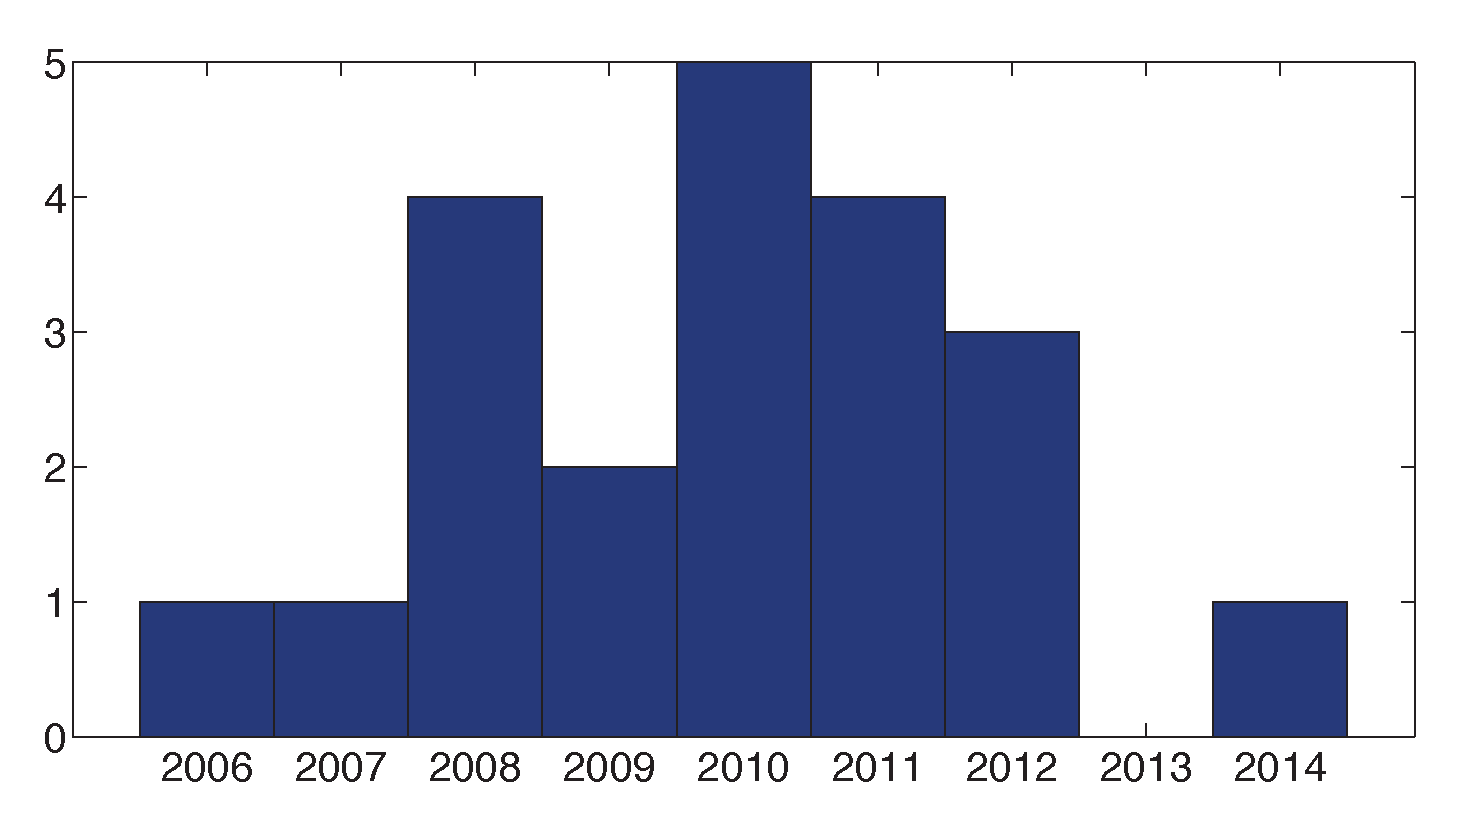
\includegraphics[width=.6\columnwidth]{../assets/papers.pdf}
		\vspace{-10pt}
		\caption{Referenced papers per year.}
	\end{figure}
	%Uitleg wat we gedaan hebben; Survey met als doel..
	%Indeling presentatie
	%Evt.: Uitleg dat we MT specifieke problemen pakken. (DB Schalen niet persé moeilijk, MT DB wel.., dat idee).
\end{frame}

\begin{frame}\frametitle{\textbf{\LARGE{\textrm{What is Multi-Tenancy}}}}
	\begin{columns}
		\column{.75\textwidth}
		\begin{itemize}
			\item No official definition! % official -> agreed upon?
			\item Tenant: Group of users sharing view.
			\item Multiple tenants on the same instance.
			\item Key subjects:
				\begin{itemize}
				\item Security
				\item Scalability \& QoS
				\item Variability
				\end{itemize}
		\end{itemize}
		\column{.25\textwidth}
		\includegraphics[width=.8\columnwidth]{images/large_questionmark.jpg}
	\end{columns}
\end{frame}

%TODO: Plaatje
\begin{frame}\frametitle{\textbf{\LARGE{\textrm{The State of Security}}}}
	\begin{itemize}
		\item Security: vital for major adoption.
		\item Main security Issues with multi-tenancy:
		\begin{itemize}
			\item Data localization.
			\item Secure data storage.
			\item Authorization and authentication.
			\item Dependence on insecure underlying technologies.
		\end{itemize}
	\end{itemize}
\end{frame}

%TODO: Plaatje
\begin{frame}\frametitle{\textbf{\LARGE{\textrm{The State of Scalability}}}}
	\begin{itemize}
		\item Multi-Tenant applications must be scalable.
		\item Subjects in the application layer:
			\begin{itemize}
				\item Estimating resource usage per tenant, per user.
				\item Tenant placement \& resource allocation.
			\end{itemize}
		\item Subjects in the data layer:
			\begin{itemize}
				\item Scalable handling of extensible schemas.
			\end{itemize}
	\end{itemize}
\end{frame}

%TODO: Plaatje
\begin{frame}\frametitle{\textbf{\LARGE{\textrm{The State of Quality of Service}}}}
	\begin{itemize}
		\item Tenants should not be able to affect other tenants.
		\item Performance requirements may differ per tenant.
		\item Subjects: % subjects about whut?
			\begin{itemize}
				\item Aggressive tenant handling.
				\item Performance isolation.
			\end{itemize}
	\end{itemize}
\end{frame}

\begin{frame}\frametitle{\textbf{\LARGE{\textrm{The State of Variability}}}}
	\setbeamercolor{palette primary}{fg=red,bg=red!85}       % Right field
	\setbeamercolor{palette secondary}{fg=red,bg=red!85}     % Middle field
	\setbeamercolor{structure}{fg=red}
	\begin{itemize}
		\item Variability is where value is added for tenants
		\item Customize anything: from logo's to complete workflows or data models
		\item Subjects:
			\begin{itemize}
				\item Levels of variability
				\item Variability modeling
				\item Techniques to realize variability
			\end{itemize}
	\end{itemize}
\end{frame}

\begin{frame}\frametitle{\textbf{\LARGE{\textrm{Research Opportunities}}}}
\end{frame}

\begin{frame}\frametitle{\textbf{\LARGE{\textrm{Research Opportunities cont'd}}}}
\end{frame}

% Reminder: "Take the pledge: Say no to “Thank you!” or “Questions?” slides."
\begin{frame}\frametitle{\textbf{\LARGE{\textrm{Questions and Discussion}}}}
	% TODO: takeaway message
\end{frame}


\end{document} 
